\chapter{Hyperparameters}
\section{K-Means}
For selecting the appropriate amount of clusters, we used an "elbow" plot in combination with the silhouette score.
\begin{enumerate}
  \item Seeds dataset: 4 clusters (see figure: \ref{hyperparameters:k-means-seeds-dataset})
  \item Heart dataset: TODO
  \item Circle dataset: 5 clusters (see figure: \ref{hyperparameters:k-means-circle-dataset})
  \item Line dataset: 4 clusters (see figure: \ref{hyperparameters:k-means-line-dataset})
  \item Skewed dataset: 4 clusters (see figure: \ref{hyperparameters:k-means-skewed-dataset})
\end{enumerate}
\begin{figure}[H]
  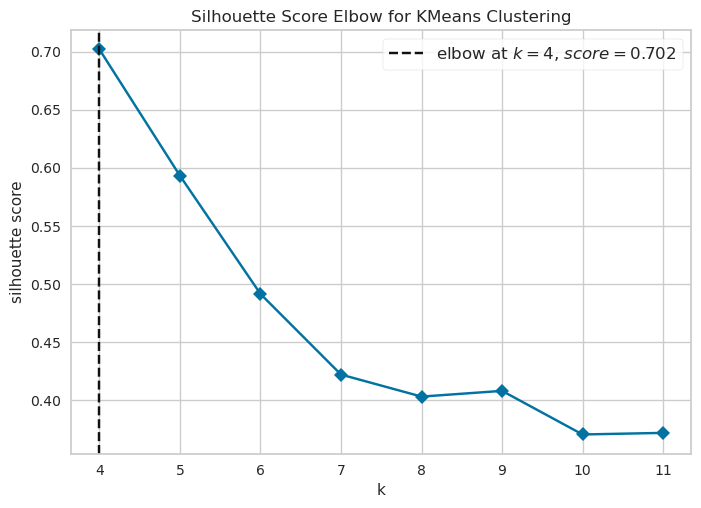
\includegraphics[width=0.6\textwidth]{Appendix/parameter-selection/selecting-k.png}
  \caption{Selecting the $k$ for K-Means for seeds dataset using the "elbow plot" using section \ref{theory:kmeans}}
  \label{hyperparameters:k-means-seeds-dataset}
\end{figure}

\begin{figure}[H]
  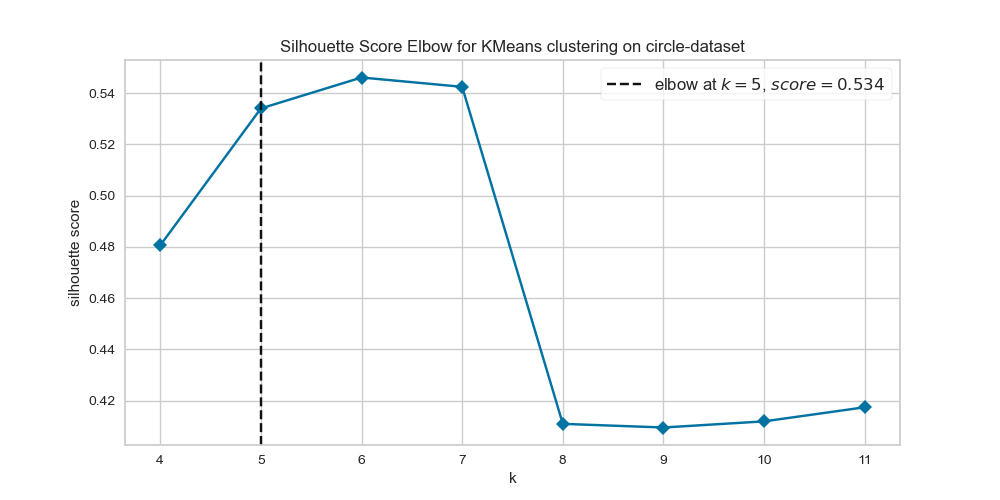
\includegraphics[width=0.6\textwidth]{Method/images/synthetic-datasets-k/circle-dataset_elbow.png}
  \caption{Selecting the $k$ for K-Means for the circle dataset using the "elbow plot" using section \ref{theory:kmeans}}
  \label{hyperparameters:k-means-circle-dataset}
\end{figure}


\begin{figure}[H]
  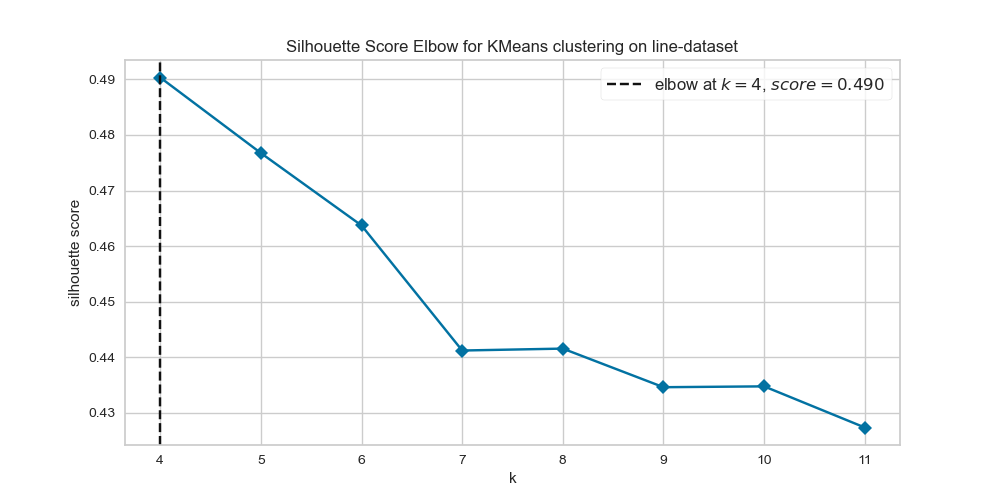
\includegraphics[width=0.6\textwidth]{Method/images/synthetic-datasets-k/line-dataset_elbow.png}
  \caption{Selecting the $k$ for K-Means for the line dataset using the "elbow plot" using section \ref{theory:kmeans}}
  \label{hyperparameters:k-means-line-dataset}
\end{figure}

\begin{figure}[H]
  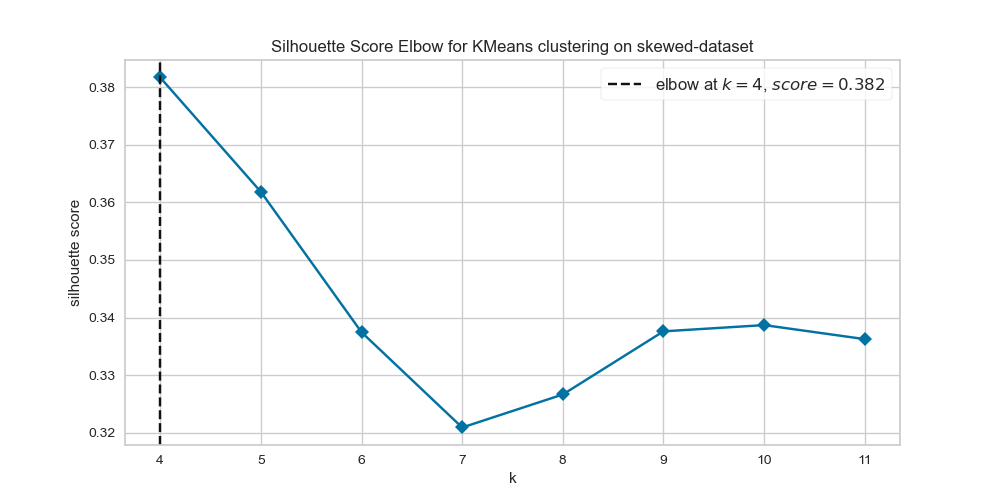
\includegraphics[width=0.6\textwidth]{Method/images/synthetic-datasets-k/skewed-dataset_elbow.png}
  \caption{Selecting the $k$ for K-Means for the skewed dataset using the "elbow plot" using section \ref{theory:kmeans}}
  \label{hyperparameters:k-means-skewed-dataset}
\end{figure}